\section{Motivation}

The research presented in this thesis is intended as a contribution to scientific research in multiscale dynamical systems. Multiscale systems often arise when a physical process is modeled mathematically. In such cases, fundamental physical conservation laws are often used to derive the differential equations governing a system at microscopic scales. It frequently happens that one seeks to understand phenomena that occur on time or space scales orders of magnitude larger than those on which the microscopic equations are derived. In theory, this does not present a problem; in order to understand macroscopic phenomena, one should simply calculate with the microscopic equations over and over until the large scales of interest are reached. In practice, things can become complicated, and the results in this thesis help address two problems that arise.

The first problem is one of computational cost. Despite advances in computational power, one cannot always take the microscopic equations and hope to simulate them for time-spans orders of magnitude larger than their intrinsic time-scales to reveal macroscopic phenomenology. To borrow from the computational mechanics community, the problem may be too ``stiff'', so that obtaining results on the scales of interest will require so many calculations at the microscopic timescales that observing macroscopic phenomena will take far too much computer time.

Another problem can arise due to noise. It is almost a given that any mathematical model of a physical system neglects certain phenomena. While it may be possible to demonstrate that the exclusion of certain effects is inconsequential over microscopic length scales, this seldom proves that these same effects can be ignored over macroscopic scales. In order to elucidate such problems, it can be fruitful to lump all unmodeled dynamics into small amplitude stochastic forcing terms. The question then becomes one of determining if and how forcing on microscopic scales is transferred to macroscopic scales. The method known as stochastic averaging directly addresses this question.

%\section{History of stochastic averaging}
%% Important papers
%%% Stratonovich
%%% Khasminskii
%%% Strook, Varadhan, Papanicolaou: the martingale problem
%%% Fredlin and Wentzell: stochastic averaging with the martingale problem
%%% Namachchivaya & Sowers: rederived classical results, extended and applied methods.

%\section{The Duffing van der Pol oscillator}
%% Toy problem

\section{Stochastic Averaging Theory}
\label{s:stochatic averaging theory}

In this section, the general formulation used to setup mechanical systems so as to make them amenable to analysis with stochastic averaging is given. The key formulas that enable the application of stochastic averaging theory to mechanical systems are then presented.

The starting point is a general form for the equations of the dynamical systems that shall be averaged. The results of stochastic averaging based on the martingale problem are then given. The section concludes by giving a precise definitions for the drift and diffusion coefficients of a stochastically averaged Markov. In addition, the domain of the reduced Markov process is fully defined.

Note that proofs are not provided in this thesis. Quite similar results were developed in \citet{namachchivaya01:_unified_approac_noisy_nonlin_mathieu_type_system} although in that publication stochastic averaging was used to reduce a system from two dimensions to one. While it is expected that for the problems presented in this thesis, where the reduction is from four dimensions to two, theoretical results will carry over in a straightforward manner, strictly speaking the stochastic averaging formulas used here should be taken as conjectures.

The mechanical systems analyzed in this thesis are governed by Hamiltonian dynamics. The Hamiltonian is nonlinear and by introducing a scaling parameter, $\epsilon$, the Hamiltonian can be expanded in powers of $\epsilon$:
\begin{equation}
\label{e:hamiltonian}
H(q,p) = H_0(q,p) + \epsilon H_1(q,p) + \epsilon^2 H_2(q,p) + \Order(\epsilon^3)
\end{equation}
with $q,p \in \Real^2$. The Hamiltonian dynamics are perturbed by a stochastic forcing function, $\sigma$, and to compensate for the energy input from forcing, a damping function, $\zeta$, is also introduced:
\begin{gather*}
dq_k = \frac{\partial H}{\partial p_k} dt,\\
dp_k = -\frac{\partial H}{\partial q_k} dt + \epsilon^2 \zeta(q,p) dt + \epsilon \sigma(q,p) dt.
\end{gather*}
Note that despite the different powers of $\epsilon$ in front of the damping and noise, these two effects ultimately have equal influence; the peculiar scaling stems from the quadratic variation of Brownian processes that affects how such processes rescale with timescale changes.

In order to remove the leading order terms of the Hamiltonian, i.e. $H_0$, a canonical transformation is used. Symbolically, the transformation can be denoted $(q_1,q_2,p_1,p_2) \mapsto (x_1,x_2,x_3,x_4)$; the conjugate pairs are $(x_1,x_3)$ and $(x_2,x_4)$. It is important to note that this transformation is time-dependent, therefore it involves a generating function \citep[\S 9.1]{goldstein80:_class}.

The dynamics of $x \equiv (x_1,x_2,x_3,x_4)$ have the form:
\begin{equation}
\label{e:perturbed dynamics}
dx^\epsilon_t = \epsilon b^1(x^\epsilon_t,t) dt + \epsilon^2 b^2(x^\epsilon_t,t) dt + \epsilon g (x^\epsilon_t, t) dt.
\end{equation}
In this equation, $b^1$ is associated with Hamiltonian dynamics, $b^2$ with damping and $g$ with stochastic forcing.

A key difference between typical stochastic averaging problems and stochastic averaging applied to mechanical systems now comes to light. Typically, stochastic averaging is applied to systems with two timescales, Equation \eqref{e:perturbed dynamics} however, contains three timescales: (i) the timescale associated with the time-dependent transformation from $(q_1,q_2,p_1,p_2) \mapsto (x_1,x_2,x_3,x_4)$; this is the shortest timescale of the system, (ii) the timescale associated with periodic motion along Hamiltonian orbits; this is an intermediate timescale and (iii) the timescale over which stochastic forcing, which is of small amplitude, has an effect; this is the longest timescale. These timescales are separated from one another by a factor of $\epsilon$. Typically, stochastic averaging would be applied to average out our intermediate timescale so as to obtain an averaged equation valid at our longest timescale. In order to arrive at such results for the problems presented in this thesis, a supplementary averaging step will be necessary. Specifically, a time averaging operator with a period equal to the period of the canonical transformation mentioned above will appear. This supplementary averaging operator is defined below.
\begin{definition}[Time averaging operator]
\label{d:Tave}
For a function $\varphi \in C^\infty(\Real^4 \times \Real)$ which is $2\pi$ periodic in its last argument, define the time averaging operator $\Tave$ by
\[
(\Tave \varphi)(x)\equiv \frac{1}{2\pi}\int_0^{2\pi} \varphi(x,t) dt.
\]
\end{definition}
Stochastic averaging with this additional time-scale was first presented in \citet{namachchivaya01:_unified_approac_noisy_nonlin_mathieu_type_system}.

\subsection{Structure of the Unperturbed System}

Having stated that stochastic averaging enables the analysis of the effects of small amplitude stochastic perturbations over long timescales, selection of the slow variables must now be considered. In the context of multiscale dynamical systems, knowing how to select good slow variables can be challenging. Recently, anistropic diffusion maps \citep{singer09:_detec} have been proposed as machinery that would help automate the discovery of slowly changing variables, however in this thesis we used the more traditional approach of relying on insight into the problem at hand for finding the slowly changing variables. For mechanical system with a Hamiltonian structure, it seems quite natural to select the Hamiltonian as a slow variable. It is the average of the Hamiltonian of Equation \eqref{e:hamiltonian} over its cyclic coordinates that gives the first integral of motion, $K$, defined as follows:
\[
K = \Tave[H_1].
\]
$K$ generates Hamiltonian dynamics. The variable $z$ will be associated with these unperturbed dynamics, so that:
\begin{equation}
\label{e:unperturbed dynamics}
\dot z = \bar \nabla K
\end{equation}
where
\[
\bar \nabla \equiv \left(\frac{\partial}{\partial z_3}, -\frac{\partial}{\partial z_1}, \frac{\partial}{\partial z_4}, -\frac{\partial}{\partial z_2}\right)
\]
A key objective of this thesis is to treat 2-D averaging problems, thus two degree of freedom systems (i.e. systems in $\Real^4$) are taken as the starting point and their reduction to 2-D is sought. The second slow variable is introduced by setting the two modes of system \eqref{e:unperturbed dynamics} to be in low-order resonance with each other. This second slow variable is akin to an angular momentum and is denoted by $I$. Thus, the two slow variables that will be part of our analysis are $K$ and $I$, we combine them in the vector $y = (K,I)$.

Before considering the dynamics of $y$, let us start by considering the geometric structure of space associated with the unperturbed system. This is important since the stochastically perturbed system evolves in the domain defined by the unperturbed system.

The main point behind the stochastic averaging method developed here is to use the geometric structure of the averaged integrable Hamiltonian problem, Equation \eqref{e:unperturbed dynamics} in order to develop an appropriate set of ``coordinates'' for studying the perturbed problem, Equation \eqref{e:perturbed dynamics}.

The simplest case one can encounter is when the Hamiltonian has a single elliptic fixed point. As illustrated in Figure \ref{f:classical reduction}, the reduced space is then a line segment. When the Hamiltonian has more than one fixed point, the notion of a reduction to a line segment is insufficient. As illustrated in Figure \ref{f:graph reduction}, the reduced space is a graph.

\begin{figure}
\begin{center}
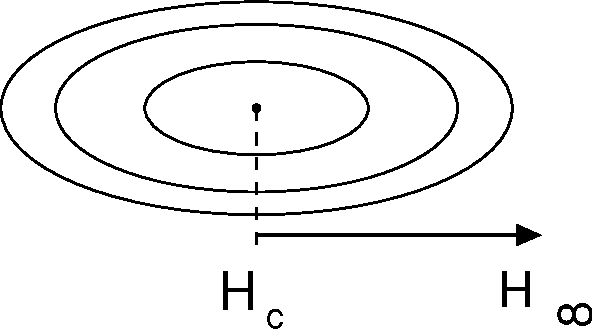
\includegraphics[width=\textwidth*7/8]{figures/classical_sa}
\caption{Depiction of the relation between the 2-D phase space of a Hamiltonian system with a single elliptic fixed point and the reduced space, a line segment.}
\label{f:classical reduction}
\end{center}
\end{figure}

\begin{figure}
\begin{center}
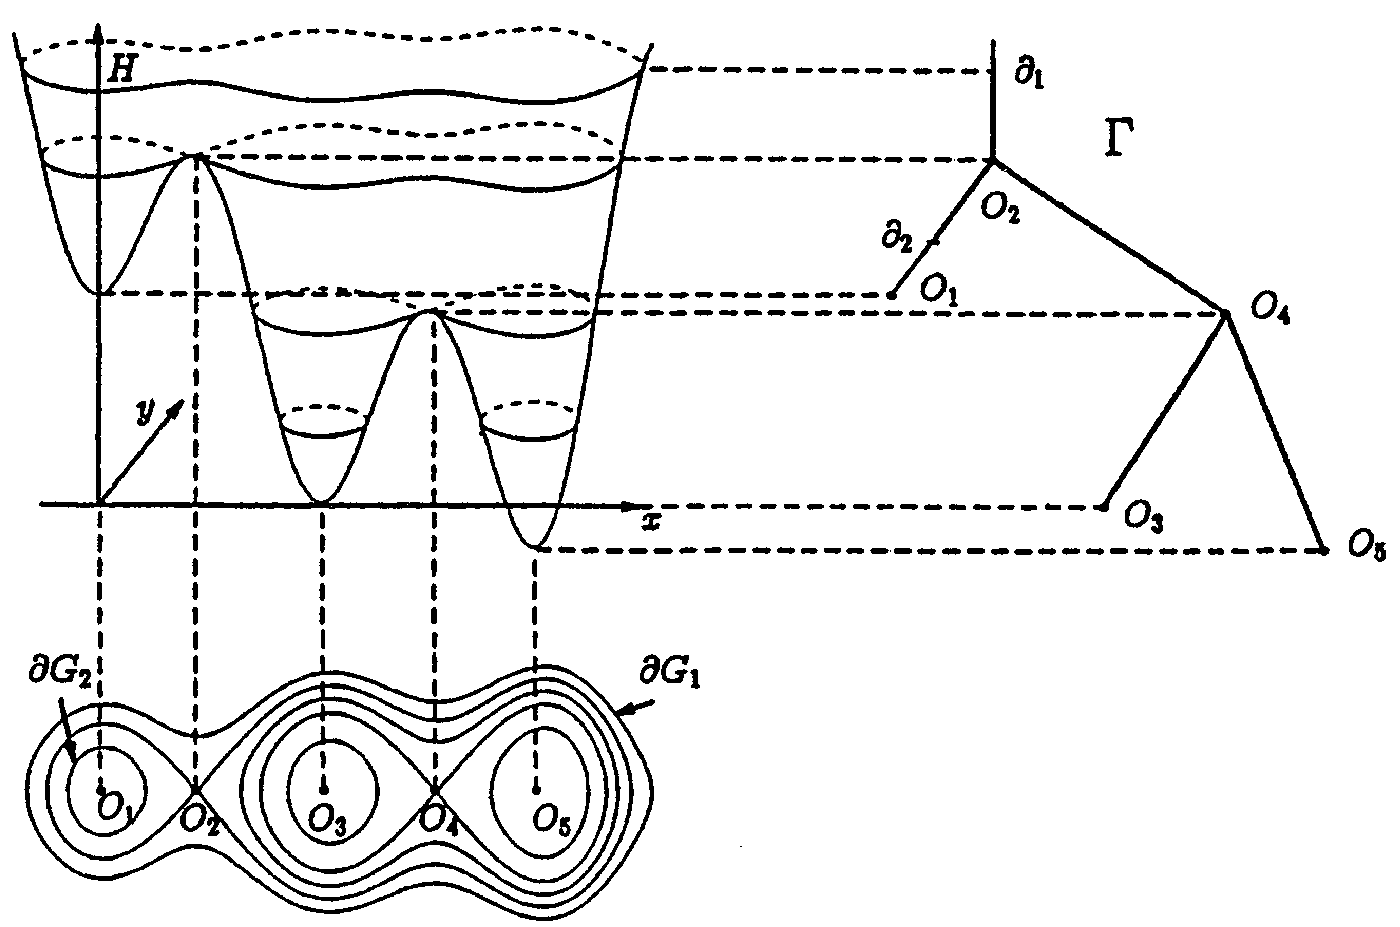
\includegraphics[width=\textwidth*7/8]{figures/graph_reduction_freidlin_weber}
\caption{Depiction of the relation between the 2-D phase space of a Hamiltonian system with multiple fixed points and the corresponding reduced graph. Figure reproduced from \citet{freidlin98:_random_pertur_nonlin_oscil}.}
\label{f:graph reduction}
\end{center}
\end{figure}

The reduced space of the problems studied in this thesis is two dimensional. Line segments seen in Figures \ref{f:classical reduction} and \ref{f:graph reduction} then become planes and the terminology of reduction on an open book \cite{freidlin04:_diffus} is introduced. Specific open book geometries will be given in \ref{s:unperturbed structure} and \ref{S:Unperturbed}, but here a general description is presented, in part to introduce notation.

The phase space of the systems we consider is composed  of elliptic and saddle fixed points, $\mathfrak{c}_i$, closed orbits with arbitrarily large values of $I$ where the process is killed $\BDY_i$ and open leaves, $\Gamma_i$ within which classical averaging results are valid. The union of these three components forms the graph of the reduced process:
\[
\Graph \equiv \bigcup_{i=1}^{N} \Gamma_i \cup \bigcup_{i=1}^{N_c}
[\mathfrak{c}_i] \cup \bigcup_{i=1}^{N_b}\BDY_i.
\]

\subsection{Main Results}

The dynamics of $y$ will deviate from those of $z$ noticeably only on time scales of order $\epsilon^{-1}$, thus time is rescaled such that $X^\epsilon_t \equiv x^\epsilon_{t/\epsilon^2}$. The fast dynamics are then governed by
\begin{equation}
\label{e:fast sde}
d X^\epsilon_t = \frac{1}{\epsilon} b^1 (X^\epsilon_t, t/\epsilon^2) dt + b^2 (X^\epsilon_t,t/\epsilon^2) dt + \frac{1}{\epsilon} g(X^\epsilon_t,t/\epsilon^2) dt
\end{equation}
and the slow dynamics are governed by
\begin{equation}
\label{e:slow sde}
dY^{\epsilon}_t = \frac{1}{\epsilon} F^1(X^\epsilon_t,t/\epsilon^2) dt + F^2(X^\epsilon_t,t/\epsilon^2) dt + \frac{1}{\epsilon} G(X^\epsilon_t,t/\epsilon^2) dt.
\end{equation}
The coefficients of the slow equation are found using the chain rule and Ito's formula (i.e. the stochastic chain rule), specifically,
% Formulas below are the standard chain rule, which is valid for real noise forcing. Do the formulas change if white noise forcing is used?
\begin{equation}
\label{e:slow sde coefficients}
\begin{aligned}
F^1_1& = \sum^4_{i = 1} \frac{\partial K}{\partial x_i} b^1_i& F^1_2& = \sum^4_{i = 1} \frac{\partial I}{\partial x_i} b^1_i\\
F^2_1& = \sum^4_{i = 1} \frac{\partial K}{\partial x_i} b^2_i& F^2_2& = \sum^4_{i = 1} \frac{\partial I}{\partial x_i} b^2_i\\
G_1& = \sum^4_{i = 1} \frac{\partial K}{\partial x_i} g_i&
G_2& = \sum^4_{i = 1} \frac{\partial I}{\partial x_i} g_i
\end{aligned}
\end{equation}
Note that $\Tave[b^1] = \bar \nabla K$, therefore
\[
\Tave[F^1_1] = \nabla K \cdot \bar \nabla K.
\]
Since the gradient and symplectic gradient produce vectors perpendicular to each other, $\Tave[F^1_1] = 0$. Similarly $\Tave[F^1_2] = 0$, therefore it starts to become evident that the dynamics of Equation \eqref{e:slow sde} are an order of $\epsilon$ slower than those of Equation \eqref{e:fast sde}.

This demonstrates that the dynamics of $Y_t^\epsilon$ are indeed slow compared to those of $X_t^\epsilon$.

For all problems treated in this thesis, it is a given that the fast process is a Markov process, which is to say a process for which the future is independent of everything but the present (delay differential equations do not satisfy this property.) Equation \eqref{e:fast sde} has a generator (\citep[\S 7.3]{oksendal98:_stoch_differ_equat}). For $\phi \in C^2(\Real^4 \times \Real)$ this generator is:
\[
(\gen^\epsilon \phi)(x,t) = \epsilon^{-1} (b^1,\nabla \phi)(x,t) + (\gen \phi)(x,t)
\]
where
\[
(\gen \phi)(x,t) = \sum_{i = 1}^4 b_i^2(x,t) \frac{\partial \phi}{\partial x_i}(x) + \frac12 \sum_{i,j=1}^4 a_{ij}(x,t) \frac{\partial^2 \phi}{\partial x_i \partial x_j}(x)
\]
where $a_{ij}(x,t) \equiv (g(x,t) g^T(x,t))_{ij}$. The theory of stochastic averaging provides the formalism required to prove that in the limit of infinitesimally small $\epsilon$, the generator for
$Y_t^\epsilon$ becomes decoupled from $X_t^\epsilon$. Effectively then, averaging becomes a method for dimensional reduction since a system in $\Real^4$ is approximated by one in $\Real^2$. Formally this result holds for infinitesimally small $\epsilon$.

The problem has now been setup to apply stochastic averaging theory. First, the results of stochastic averaging theory are stated and then the methods used to arrive at those results is explained. It must be noted that proofs for the results given below are not provided in this thesis, although in \citet{namachchivaya01:_unified_approac_noisy_nonlin_mathieu_type_system} similar results are proved. The principal difference between results in that reference and those used in this thesis is that in the reference, reduction from $\Real^2 \to \Real$ is analyzed, whereas here, the case of reduction from $\Real^4 \to \Real^2$ is treated. While this difference should not lead to significant changes, strictly speaking, the stochastic averaging formulas given below should be termed conjectures.

To begin, an averaging operator is defined.
\begin{definition}[Hamiltonian orbit averaging operator]
\label{d:Aave}
For a function $\varphi \in C^\infty(\Real^4)$, define averaging operator acting over Hamiltonian orbits, $\Aave$ by
\[
(\Aave \varphi) (y) \equiv \frac{1}{\period(y)} \int_0^{\period(y)} \varphi(z_s(x)) ds
\]
where $T(y)$ is the period associated with a Hamiltonian orbit.
\end{definition}

The reduced Markov process is defined in terms of its drift and diffusion coefficients. These two quantities are given by the following definition.
\begin{definition}[Averaged drift \& diffusion coefficients]
\begin{gather}
\mathfrak{b}_i(y) \equiv \left(\Aave \left(\Tave \left(F_i^2 + \mathfrak{f}_i + \mathfrak{g}_i\right)\right)\right)(y)\label{e:drift}\\
\Aa_{ij}(y) \equiv \left(\Aave \left(\Tave \left(\sigma\sigma^T\right)_{ij}\right)\right)(y)\label{e:diffusion}
\end{gather}
for $i,j = 1,2$, where
\[
\mathfrak f_i(x,t) \equiv \sum_{j=1}^4 \frac{\partial F_i^1(x,t)}{\partial x_j} \tilde f_j^1(x,t)
\]
\[
\tilde f_i^1 (x,t) \equiv \int_0^t \left\{b_i^1 (x,s) - \Tave_s (b_i^1(x,s)) \right\} ds\\
\]
\[
\mathfrak g_i(x,t) \equiv \int_{-\infty}^0 \Expectation \left[ \frac{\partial G_i (x,t,\xi_t)}{\partial x_j} g_j(x,t+\tau,\xi_{t+\tau}) \right] d\tau
\]
\[
\left(\sigma\sigma^T\right)_{jk}(x,t) \equiv \int_{-\infty}^\infty
\Expectation \left[G_j(x,t,\xi_t) G_k (x, t + \tau, \xi_{t+\tau}) \right] d\tau
\]
\end{definition}
It's worth pointing out that classical stochastic averaging theory, i.e. \citet{khas'minskii68:_ito} is sufficient to provide these results since they hold within the leaves of the reduced domain, where one need not deal with fixed points and infinite periods.

\begin{definition}[Generator of the reduced Markov process]
\label{d:reduced generator}
The generator of the reduced Markov process is, for a function $f \in
C^2(\Real^2)$,
\[
(\gen_i^\dagger f)(y) = \sum_{j=1}^2
\mathfrak{b}^i_j(y) \frac{\partial f(y)}{\partial y_j} +
\frac12 \sum_{j,k = 1}^2 \mathfrak{a}^i_{jk}(y)
\frac{\partial^2 f(y)}{\partial y_j \partial y_k}
\]
$\mathfrak{b}$ is the drift coefficient and $\mathfrak{a}$ the diffusion coefficient. The domain of the generator of the process evolving on a $\mathfrak{G}$ with $n$ leaves is defined by
\begin{multline}
\mathfrak{D}_\mathfrak{G}^\dagger = \{f \in C(\mathfrak{G}) \cap
C^2(\bigcup_{i=1}^n \Gamma_i): \lim_{y \to \mathfrak c_i} (\gen^\dagger_i f)(y) \text{ exists}, \lim_{y \to \BDY_i} (\gen^\dagger_i f)(y) = 0 \quad \forall\, i,\\
\sum_{i=1}^n \{\pm\} \sum_{j=1}^2 \Bigl\{\sum_{k=1}^2
\mathring{\mathfrak a}^i_{jk}(\mathcal{O}) \frac{\partial f}{\partial
y_k}\bigg|_\mathcal{O} \Bigr\} \cdot \nu_j(\mathcal O) =0 \}
\label{e:generator domain}
\end{multline}
where $\mathring{\mathfrak{a}}$ denotes the same coefficient as in equation \eqref{e:diffusion} except that the $\Aave$-averaging operator excludes division by the period and $\mathcal O$ denotes the gluing vertex.
\end{definition}

The sum involving $\mathring{\mathfrak a}$ constitutes the gluing condition. An intuitive interpretation of the gluing condition is provided in \citet{namachchivaya01:_unified_approac_noisy_nonlin_mathieu_type_system}. This interpretation is extended to two-dimensions here. Define
\[
\alpha = \sum_{i=1}^n \lVert \mathring{\mathfrak a}^i(\mathcal{O}) \rVert.
\]
Suppose the limiting process starts on the page $\Gamma_1$. It will evolve according to $\gen_1^\dagger$ until it hits the gluing vertex. The process will then return to page $\Gamma_1$ with probability $\lVert \mathring{\mathfrak a}^1(\mathcal{O}) \rVert/\alpha$ and it will go to page $\Gamma_i$ with probability $\lVert \mathring{\mathfrak a}^i(\mathcal{O}) \rVert/\alpha$.

Now, a sketch is given for the proof that $\gen^\dagger$ is the generator of a Markov process and Equation \eqref{e:generator domain} its domain.
% FIXME Wiener vs. Brownian process
The Wiener process of the fast process given in Equation \eqref{e:fast sde} is given on the \emph{original} probability space, $(\Omega^o,\filt^o,\prob^o)$, where $\Omega^o$ is the event space, $\filt^o$ the filtration, and $\prob^o$ the probability measure. A \emph{canonical} space is introduced so as to transfer the dependence on $\epsilon$ from the process onto the measure. The original and canonical spaces are related by
\[
\prob^\epsilon(A) \equiv \prob^o(X^\epsilon \in A), \quad A \in B(\Omega)
\]
where $B(\Omega)$ denotes the space of Borel measures on $\Omega$.

The martingale problem is used because it gives an alternative formulation for the existence and uniqueness of weak solutions of stochastic differential equations (SDEs). Classical existence and uniqueness properties of are proved using Holder continuity of the SDE's coefficient, but such conditions are too strong to deal with the topology of the reduced space, which consists of leaves with edges that have singularities due to the homoclinic structure of the fast deterministic dynamics. Formally, the martingale problem is stated as follows \citep{rogers00:_diffus_markov}. Denote an SDE by:
\[
dX = b(X,t) dt + \sigma(X,t) dW
\]
Suppose $X$ is a weak solution to this equation starting at $y \in \Real^n$. Let $\prob^y$ be the law of $X$; $\prob^y$ is a probability measure on $(\Omega^n,\filt_t^n)$. Then $\prob^y$ has the following properties
\begin{enumerate}
\item $\prob^y(x_0 = y) = 1$
\item under $\prob^y$, for each $f \in C^\infty(\real^n)$
\[
M_t^f \equiv f(x_t) - f(x_0) - \int_0^t L f(x,s) ds
\]
where $L$ denotes the SDE's generator, is an $\filt_t^n$ martingale.
\end{enumerate}

For the fast process, $X_t^\epsilon$, the existence and uniqueness of weak solutions is assured by the fact that \eqref{e:fast sde} is a well-behaved SDE. Thus, by the martingale problem we can state that, for $f \in C^2(\Real^4 \times \Real)$ a function $2\pi$-periodic in its last argument,
\[
M_t^{f,\epsilon} \equiv f(X_t,t/\epsilon^2) - \int_0^t \epsilon^{-2} \frac{\partial f}{\partial s}(X_s,s/\epsilon^2) + (\gen^\epsilon f)(X_s,s/\epsilon^2) ds,
\]
% FIXME Where does the \order(\epsilon^{-2}) term come from?
is a martingale with respect to the filtration ${\filt_t; t \geq 0}$ under the probability measure $\prob^\epsilon$. An alternative form of the martingale problem is used in proofs \citep{ethier86:_markov_process}. If $0 \leq r_1 < r_2 \dots < r_n \leq s < t$ and ${\phi_j; j = 1,2 \dots n} \in C_b(\Real^n)$, then
\begin{multline*}
\Expectation^\epsilon \Big[\Big\{f(X_t) - f(X_s) - \int_s^t \epsilon^{-2} \frac{\partial f}{\partial s}(X_u,u/\epsilon^2) \\
+ (\gen^\epsilon f)(X_u,u/\epsilon^2) du\Big\} \prod_{j=1}^{n} \phi_j(X_{r_j})\Big] = 0.
\end{multline*}
This form of the martingale property relies on the fact that functions of the form $\prod_{j=1}^n \phi_j(X_{r_j})$ generate $\filt_s$.

Stochastic averaging theory show that the law of the reduced process, $Y^\epsilon_t$, converges to a unique limit. This is also stated in a canonical space. $Y^\epsilon_t$ takes values in $\Graph$. The event space is $\Omega^\dagger \equiv C([0,\infty),\Graph)$, the filtration is $\filt^\dagger$ and the canonical probability measure is defined by
\[
\prob^{\epsilon,\dagger} \equiv \prob^{\epsilon}(Y \in A),\quad A \in B(\Omega^\dagger).
\]
Stochastic averaging theory is used to prove the existence and uniqueness of the limit
\begin{equation}
\label{e:limit def}
\prob^\dagger \equiv \lim_{\epsilon \to 0} \prob^{\epsilon,\dagger}.
\end{equation}
Formally, the main theorem of stochastic averaging is stated as follows. $\prob^{\epsilon,\dagger}$ tends to a unique solution $\prob^\dagger$ of the martingale problem with generator $\gen^\dagger$ and with initial condition $\delta_{y_0}$. This means $\prob(Y_0^\dagger = Y_0) = 1$, and if $f \in \mathfrak{D}_\mathfrak{G}^\dagger$, $0 \leq r_1 < r_2 \dots < r_n \leq s < t$ and ${\phi_j^\dagger; j = 1,2 \dots n} \in C(\Graph)$, then
\begin{equation}
\label{e:sa main}
\Expectation^\dagger \left[\left\{f(Y_t^\dagger) - f(Y_s^\dagger) - \int_s^t (\gen^\dagger f)(Y_u^\dagger) du\right\} \prod_{j=1}^{n} \phi_j^\dagger(Y_{r_j}^\dagger)\right] = 0.
\end{equation}

% FIXME \gen^\dagger vs. \gen^\dagger_i
To prove that $\gen^\dagger$ is the generator of a Markov process, the first step is to show the reduced probability measure, $\prob^{\epsilon,\dagger}$ is tight in the Prohorov topology on $B(\Omega^\dagger)$. Then, by Prokhorov's theorem, there exists at least one cluster point in the weak topology of probability measures on $\Omega^\dagger$.

Based on definition \eqref{e:limit def}, \eqref{e:sa main} can be stated as
\[
\lim_{\epsilon \to 0} \Expectation^{\epsilon,\dagger} \left[\left\{f(Y_t^\dagger) - f(Y_s^\dagger) - \int_s^t (\gen^\dagger f)(Y_u^\dagger) du\right\} \prod_{j=1}^{n} \phi_j^\dagger(Y_{r_j}^\dagger)\right] = 0
\]
and reverting back to the unreduced process, the above can be stated as
\[
\lim_{\epsilon \to 0} \Expectation^\epsilon \left[\left\{f(Y_t) - f(Y_s) - \int_s^t (\gen^\dagger f)(Y_u) du\right\} \prod_{j=1}^{n} \phi_j(Y_{r_j})\right] = 0.
\]
In the original canonical space, it's known that, if $y = \mathcal R(x,y)$,
\[
\Expectation^\epsilon \left[\left\{f(Y_t) - f(Y_s) - \int_s^t (\gen^\epsilon (f \circ \mathcal R))(X_u) du\right\} \prod_{j=1}^{n} \phi_j(X_{r_j})\right] = 0
\]
for all $\epsilon > 0$. This demonstrates that the bulk of the work that needs to be performed to prove stochastic averaging results is to show
\[
\lim_{\epsilon \to 0} \Expectation \left[\left| \left(\int_0^t (\gen^\epsilon (f \circ \mathcal R))(X_s) - (\gen^\dagger f)(Y_s)\right) du \right|\right] = 0.
\]
Denoting
\[
(\gen^\epsilon (f \circ \mathcal R))(x,t) = L^\epsilon_1(x,t) + L^\epsilon_2(x,t)
\]
where
\[
\begin{aligned}
L^\epsilon_1(x,t) &\equiv (\gen K)(x,t) \frac{\partial f^\epsilon}{\partial K} (K(x),I(x)) + (\gen I)(x,t)\frac{\partial f^\epsilon}{\partial I} (K(x),I(x))\\
&\quad + \frac12 \Big\{\langle dK,dK \rangle(x,t) \frac{\partial^2 f^\epsilon}{\partial k^2} (K(x),I(x))\\
&\quad + \langle dI,dI \rangle(x,t) \frac{\partial^2 f^\epsilon}{\partial i^2} (K(x),I(x))\Big\}\\
&\quad + \langle dK,dI \rangle(x,t) \frac{\partial^2 f^\epsilon}{\partial k \partial i} (K(x),I(x))\\
\end{aligned}
\]
and
\begin{multline*}
L^\epsilon_2(x,t) \equiv \frac{1}{\epsilon} \Big\{( b^1, \nabla K)(x,t)\frac{\partial f^\epsilon}{\partial k}(K(x),I(x))\\
+ (b^1, \nabla I)(x,t)\frac{\partial f^\epsilon}{\partial i}(K(x),I(x))\Big\}
\end{multline*}
for all $x \in \Real^4$ and $t \ge 0$. The fastest variation is the oscillation of coefficients, which has period $\epsilon^2$; the second-fastest variation is the motion around the orbits of $z$; these oscillations have period $\epsilon$. Thus we should have
\[
\int_0^t L^\epsilon_1(X_u,u/\epsilon^2)du \approx \int_0^t (\Tave L^\epsilon_1)(X_u)du \approx \int_0^t(\Aave \Tave L^\epsilon_1)(K(X_u),I(X_u)) du.
\]
It should be possible to prove this using standard averaging techniques, as was done for reduction from $\Real^2 \to \Real$ in \citet{namachchivaya01:_unified_approac_noisy_nonlin_mathieu_type_system}.
The analysis of $L^\epsilon_2$ is a bit more delicate since it contains large fluctuations, which are of order one on average.

\section{Thesis Outline}

The remainder of this thesis is organized as follows. Chapter \ref{c:oscillator} applies stochastic averaging techniques to a resonant periodically driven noisy oscillator. This is problem where the original system is two-dimensional and the reduced system is one dimensional. Thus the averaging analysis can be done without recourse to numerical techniques. In this sense, Chapter \ref{c:oscillator} serves as an introductory example. This chapter is self-contained.

In Chapter \ref{c:sgwaves} a model of surface wave motion will be analyzed. This is perhaps the most challenging application of stochastic averaging in this thesis. The first step is to transform partial differential equations into an infinite system of ordinary differential equations. The graph of the reduced process has a relatively complicated geometry and in order to calculate averaged drift and diffusion coefficients, numerical algorithms are devised.

In Chapter \ref{c:autoparametric} an autoparametric oscillator model will be analyzed. The level of complexity of this problem is similar to the wave motion problem, however more calculations can be done analytically, simplifying the analysis slightly.

In Chapter \ref{c:pdf}, the main results of this thesis are developed. Stationary probability density solutions are given for the surface wave and autoparametric problems. These solutions are found with a finite-element method (FEM). In Chapter \ref{c:pdf}, a sample path method is also developed to solve the Fokker--Planck equation. This serves to validate the FEM.

Chapter \ref{c:conclusions} concludes the thesis. In that chapter, results are summarized and possible extensions to the work in this thesis are presented.

%% Classical vs. non-standard stochastic averaging: 2-D problems, third time scale, bifurcations and martingale problem and gluing condition

%%% Local Variables: 
%%% mode: latex
%%% TeX-master: "main"
%%% End: 
